% !TeX root = ../../../main.tex
\section{Pianificazone} \label{_pianificazione}
Per riuscire a portare a termine il progetto entro le scadenze prefissate il gruppo ha deciso di suddividere il lavoro in 7 fasi. Ognuna di queste è poi suddivisa in ulteriori periodi di tempo più brevi in cui ci si concentrerà prevalentemente sullo svolgimento di piccole parti, che poi porteranno a realizzare il prodotto finito.\\
Di seguito vengono elencate le fasi che si andranno a percorrere. Esse vengono inserite temporalmente tra le revisioni di progetto, riportate in grassetto, in modo da avere più chiara la pianificazione.
\begin{enumerate}
    \item []
          \begin{itemize}
              \item [] \textbf{Formazione del gruppo}
          \end{itemize}
    \item \hyperref[_pianificazioneAnalisiDeiRequisiti]{Analisi dei requisiti};
    \item \hyperref[_pianificazioneConsolidamentoDeiRequisiti]{Consolidamento dei requisiti};
          \begin{itemize}
              \item [] \textbf{Revisione dei requisiti}
          \end{itemize}
    \item \hyperref[_pianificazioneProgettazioneTechnologyBaseline]{Progettazione della technology baseline};
    \item \hyperref[_pianificazioneCodificaPoC]{Progettazione e codifica proof of concept};
          \begin{itemize}
              \item [] \textbf{Revisione di Progettazione}
          \end{itemize}
    \item \hyperref[_pianificazioneProgettazioneCompletaImplementazione]{Progettazione completa e implementazione};
          \begin{itemize}
              \item [] \textbf{Revisione di qualifica}
          \end{itemize}
    \item \hyperref[_pianificazioneTermineImplementazione]{Termine implementazione e raffinamento generale};
    \item \hyperref[_pianificazioneValidazioneCollaudo]{Validazione e collaudo}.
          \begin{itemize}
              \item [] \textbf{Revisione di accettazione}
          \end{itemize}
\end{enumerate}

%-------------- FASE Analisi dei requisiti --------------

\subsection{Analisi dei requisiti} \label{_pianificazioneAnalisiDeiRequisiti}
\begin{itemize}
    \item []\textbf{Inizio:} 2020-11-20
    \item []\textbf{Fine:} 2021-01-11
    \item []\textbf{Descrizione:} creare un way of working all'interno del gruppo, effeturare l'analisi dei requisiti del capitolato scelto e produrre la documentazione necessaria per la revisione dei requisiti.
\end{itemize}

\subsubsection{Ruoli attivi}
Durante questa fase saranno presenti i seguenti ruoli:
\begin{itemize}
    \item Responsabile;
    \item Amministratore;
    \item Analista;
    \item Verificatore.
\end{itemize}

\subsubsection{Periodi e attività}

\paragraph[Primo periodo]{Primo periodo - \textnormal{Studio dei capitolati}}
\begin{itemize}
    \item [] \textbf{Inizio:} 2020-11-20
    \item [] \textbf{Fine:} 2020-12-06
    \item [] \textbf{Attività}
          \begin{itemize}
              \item \textbf{Ricerca:} individuazione e studio di strumenti utili al gruppo per lo svolgimento della prima fase del progetto;
              \item \textbf{Normazione:} scelta di regole da utilizzare durante il progetto per poter svolgere il lavoro in modo uniforme, in particolare riguardanti la documentazione, verifica e gestione della configurazione;
              \item \textbf{Analisi dei capitolati:} studio individuale dei capitolati con successiva discussione collettiva per individuare punti a favore e contro di ognuno di essi indirizzando la scelta su pochi;
              \item \textbf{Studio di fattibilità:} redazione del documento sulla base di quanto emerso dall'analisi dei capitolati;
              \item \textbf{Pianificazione:} pianificazione delle attività da svolgere in questa prima fase;
              \item \textbf{Analisi di qualità:} analisi di metriche per garantire la qualità della documentazione.
          \end{itemize}
\end{itemize}

\paragraph[Secondo periodo]{Secondo periodo - \textnormal{Normazione e scelta del capitolato}}
\begin{itemize}
    \item [] \textbf{Inizio:} 2020-12-07
    \item [] \textbf{Fine:} 2020-12-21
    \item [] \textbf{Attività}
          \begin{itemize}
              \item \textbf{Scelta del capitolato:} decisione definitiva sul capitolato da svolgere in base allo studio di fattibilità prodotto nel periodo precedente;
              \item \textbf{Normazione:} scelta di regole da utilizzare durante lo svolgimento del progetto riguardanti i processi primari, organizzativi e di supporto;
              \item \textbf{Ricerca:} studio del capitolato scelto individuando ed approfondendo le tecnologie richieste;
              \item \textbf{Analisi di qualità:} individuazione ed analisi di metriche per garantire la qualità del prodotto;
              \item \textbf{Verifica:} controllo della qualità dei prodotti sviluppati nel primo periodo e in quello corrente.
          \end{itemize}
\end{itemize}

\paragraph[Terzo periodo]{Terzo periodo - \textnormal{Pianificazione e analisi dei casi d'uso}}
\begin{itemize}
    \item [] \textbf{Inizio:} 2020-12-22
    \item [] \textbf{Fine:} 2020-12-31
    \item [] \textbf{Attività}
          \begin{itemize}
              \item \textbf{Normazione:} completamento delle parti mancanti, e revisione dell'intero documento;
              \item \textbf{Analisi dei casi d'uso:} analisi del prodotto e dei relativi casi d'uso, confrontandosi anche con il proponente;
              \item \textbf{Analisi dei rischi:} individuazione ed analisi dei rischi che possono incorrere durante lo svolgimento del progetto;
              \item \textbf{Pianificazione:} pianificazione delle attività da svolgere nelle fasi successive;
              \item \textbf{Verifica:} controllo della qualità dei prodotti sviluppati in questo periodo;
              \item \textbf{Ricerca:} studio autonomo degli strumenti e tecnologie da utilizzare nello svolgimento del progetto.
          \end{itemize}
\end{itemize}

\paragraph[Quarto periodo]{Quarto periodo - \textnormal{Analisi dei requisiti e piano di qualità}}
\begin{itemize}
    \item [] \textbf{Inizio:} 2021-01-01
    \item [] \textbf{Fine:} 2021-01-11
    \item [] \textbf{Attività}
          \begin{itemize}
              \item \textbf{Analisi dei requisiti:} analisi del prodotto e dei requisiti espliciti e impliciti che vengono richiesti;
              \item \textbf{Piano di qualità:} completare la redazione del piano di qualifica definendo e aggiornando le metriche che vengono utilizzate durante lo svolgimento del progetto;
              \item \textbf{Pianificazione:} aggiornamento della pianificazione in seguito all'analisi svolta fin'ora;
              \item \textbf{Stesura lettera di presentazione;}
              \item \textbf{Verifica:} controllo della qualità dei prodotti sviluppati in questo periodo;
              \item \textbf{Ricerca:} studio autonomo degli strumenti e tecnologie da utilizzare nello svolgimento del progetto.
          \end{itemize}
\end{itemize}
\begin{figure}[H]
    \centering
    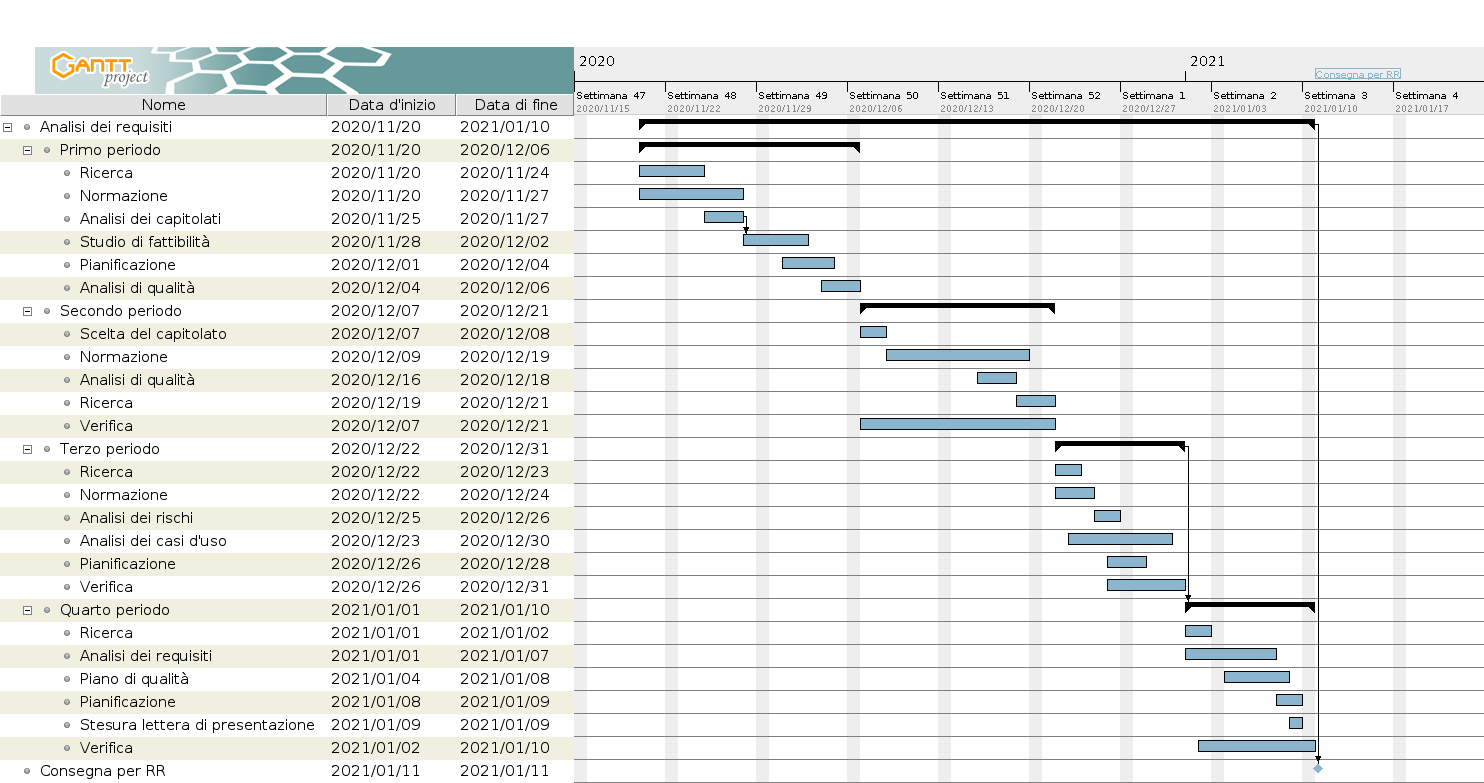
\includegraphics[width=1\linewidth]{res/images/pianificazione/analisi_dei_requisiti.png}
    \caption{Diagramma di Gantt della fase di Analisi dei requisiti}
    \label{fig:_Gantt analisi dei requisiti}
\end{figure}

%-------------- FASE Consolidamento dei requisiti --------------

\subsection{Consolidamento dei requisiti} \label{_pianificazioneConsolidamentoDeiRequisiti}
\begin{itemize}
    \item []\textbf{Inizio:} 2021-01-12
    \item []\textbf{Fine:} 2021-01-18
    \item []\textbf{Descrizione:} creare la presentazione in vista della RR.
\end{itemize}

\subsubsection{Ruoli attivi}
Durante questa fase saranno presenti i seguenti ruoli:
\begin{itemize}
    \item Responsabile;
    \item Amministratore;
    \item Analista;
    \item Verificatore.
\end{itemize}

\subsubsection{Periodi e attività}

\paragraph[Primo periodo]{Primo periodo - \textnormal{Preparazione presentazione}}
\begin{itemize}
    \item [] \textbf{Inizio:} 2021-01-12
    \item [] \textbf{Fine:} 2021-01-15
    \item [] \textbf{Attività}
          \begin{itemize}
              \item \textbf{Preparazione presentazione:} preparazione della presentazione per la revisione dei requisiti;
              \item \textbf{Verifica:} verifica della presenza di eventuali errori nella presentazione.
          \end{itemize}
\end{itemize}

\paragraph[Secondo periodo]{Secondo periodo - \textnormal{Ulteriore revisione dei requisiti}}
\begin{itemize}
    \item [] \textbf{Inizio:} 2020-01-16
    \item [] \textbf{Fine:} 2020-01-18
    \item [] \textbf{Attività}
          \begin{itemize}
              \item \textbf{Analisi dei requisiti:} revisione ed eventuale aggiornamento dei requisiti;
              \item \textbf{Studio individuale:} studio individuale di tutta la documentazione prodotta, con il focus sull'analisi dei requisiti.
          \end{itemize}
\end{itemize}

\begin{figure}[H]
    \centering
    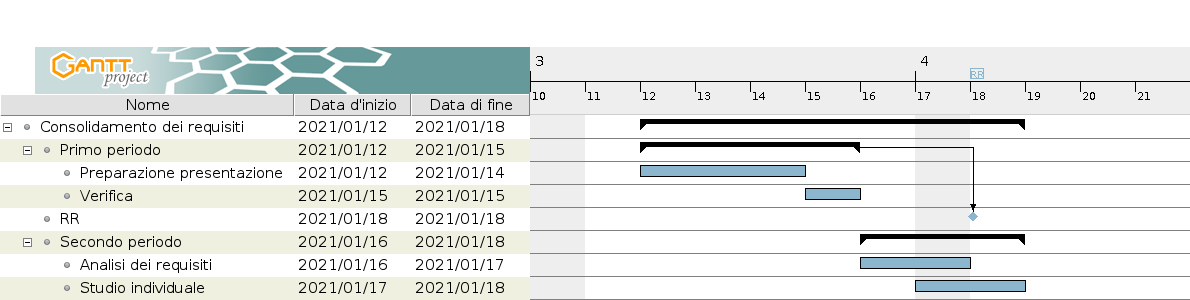
\includegraphics[width=1\linewidth]{res/images/pianificazione/consolidamento_dei_requisiti.png}
    \caption{Diagramma di Gantt della fase di Consolidamento dei requisiti}
    \label{fig:_Gantt consolidamento dei requisiti}
\end{figure}

%-------------- REVISIONE DEI REQUISITI --------------

%-------------- FASE Progettazione della technology baseline --------------

\subsection{Progettazione della technology baseline} \label{_pianificazioneProgettazioneTechnologyBaseline}
\begin{itemize}
    \item []\textbf{Inizio:} 2021-01-19
    \item []\textbf{Fine:} 2021-02-06
    \item []\textbf{Descrizione:} sistemare i documenti svolti fin'ora e progettazione dell'architettura del prodotto e di una POC.
\end{itemize}

\subsubsection{Ruoli attivi}
Durante questa fase saranno presenti i seguenti ruoli:
\begin{itemize}
    \item Responsabile;
    \item Amministratore;
    \item Analista;
    \item Progettista;
    \item Verificatore.
\end{itemize}

\subsubsection{Periodi e attività}

\paragraph[Primo periodo]{Primo periodo - \textnormal{Miglioramento documenti con indicazioni ricevute}}
\begin{itemize}
    \item [] \textbf{Inizio:} 2021-01-19
    \item [] \textbf{Fine:} 2021-01-23
    \item [] \textbf{Attività}
          \begin{itemize}
              \item \textbf{Normazione:} revisione ed eventuale aggiornamento delle norme di progetto;
              \item \textbf{Piano di qualità:} revisione ed eventuale aggiornamento del piano di qualifica;
              \item \textbf{Analisi dei requisiti:} revisione ed eventuali modifiche in base al feedback ricevuto dai committenti;
              \item \textbf{Verifica:} controllo della qualità dei prodotti sviluppati in questo periodo.
          \end{itemize}
\end{itemize}

\paragraph[Secondo periodo]{Secondo periodo - \textnormal{Progettazione architetturale}}
\begin{itemize}
    \item [] \textbf{Inizio:} 2021-01-24
    \item [] \textbf{Fine:} 2021-02-05
    \item [] \textbf{Attività}
          \begin{itemize}
              \item \textbf{Progettazione:} progettazione architetturale e del proof of concept;
              \item \textbf{Pianificazione:} aggiornamento della pianificazione delle fasi successive;
              \item \textbf{Ricerca:} studio sul funzionamento degli strumenti e delle tecnologie che verranno utilizzate (Es. AWS);
              \item \textbf{Verifica:} controllo della qualità dei prodotti sviluppati in questo periodo.
          \end{itemize}
\end{itemize}

\begin{figure}[H]
    \centering
    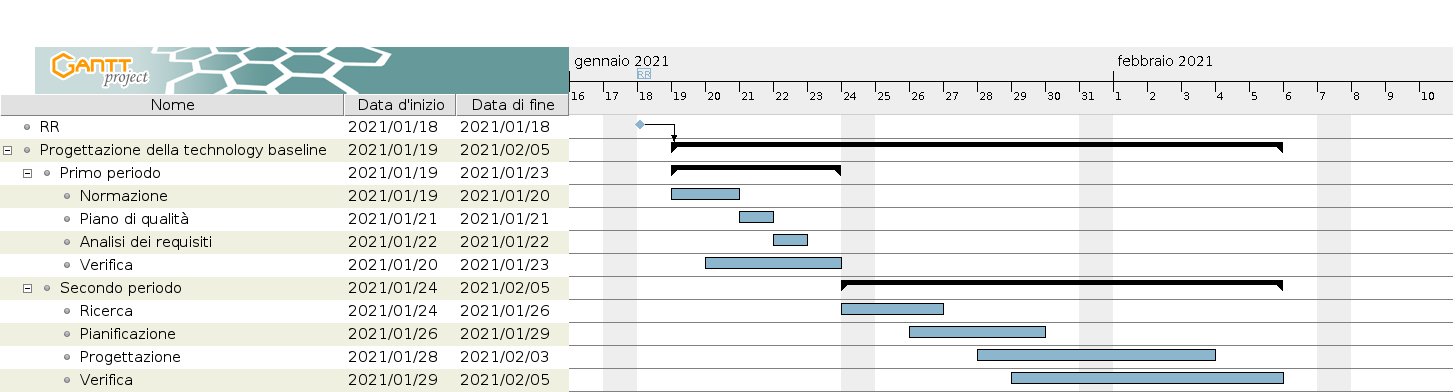
\includegraphics[width=1\linewidth]{res/images/pianificazione/progettazione_della_technology_baseline.png}
    \caption{Diagramma di Gantt della fase di Progettazione della technology baseline}
    \label{fig:_Gantt progettazione della technology baseline}
\end{figure}

%-------------- FASE Progettazione e codifica del proof of concept --------------

\subsection{Progettazione e codifica del proof of concept} \label{_pianificazioneCodificaPoC}
\begin{itemize}
    \item []\textbf{Inizio:} 2021-02-06
    \item []\textbf{Fine:} 2021-03-01
    \item []\textbf{Descrizione:} continuare la progettazione e implementare il proof of concept.
\end{itemize}

\subsubsection{Ruoli attivi}
Durante questa fase saranno presenti i seguenti ruoli:
\begin{itemize}
    \item Responsabile;
    \item Amministratore;
    \item Analista;
    \item Progettista;
    \item Programmatore;
    \item Verificatore.
\end{itemize}

\subsubsection{Periodi e attività}

\paragraph[Incremento I]{Incremento I - \textnormal{Progettazione e codifica delle componenti del PoC}}
\begin{itemize}
    \item [] \textbf{Inizio:} 2021-02-06
    \item [] \textbf{Fine:} 2021-02-21
    \item [] \textbf{Attività}
          \begin{itemize}
              \item \textbf{Analisi tecnologie da utilizzare;}
              \item \textbf{Progettazione;}
              \item \textbf{Codifica:} codifica del proof of concept;
              \item \textbf{Verifica:} controllo della qualità dei prodotti sviluppati in questo periodo.
          \end{itemize}
\end{itemize}

\begin{figure}[H]
    \centering
    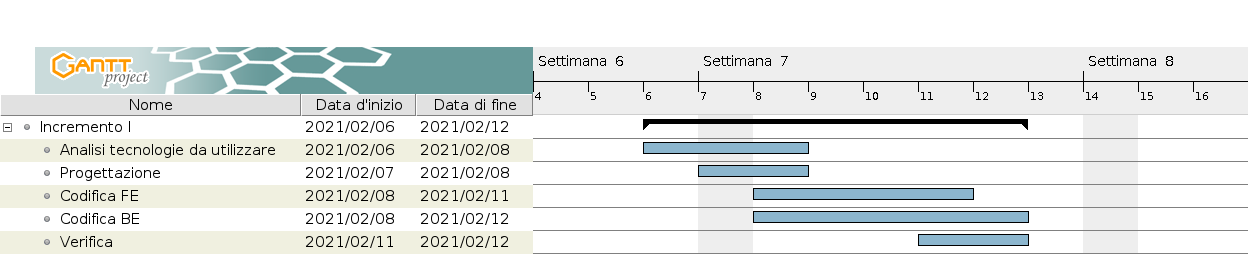
\includegraphics[width=1\linewidth]{res/images/pianificazione/incremento_1.png}
    \caption{Diagramma di Gantt dell'incremento I}
    \label{fig:_Gantt incremento I}
\end{figure}

\paragraph[Incremento II]{Incremento II - \textnormal{Raffinamento del PoC}}
\begin{itemize}
    \item [] \textbf{Inizio:} 2021-02-22
    \item [] \textbf{Fine:} 2021-03-01
    \item [] \textbf{Attività}
          \begin{itemize}
              \item \textbf{Progettazione;}
              \item \textbf{Codifica:} fine codifica e raffinamento del proof of concept;
              \item \textbf{Aggiornamento della pianificazione;}
              \item \textbf{Preparazione presentazione:} preparazione della presentazione per la revisione di progettazione;
              \item \textbf{Stesura lettera di presentazione;}
              \item \textbf{Verifica:} controllo della qualità dei prodotti sviluppati in questo periodo.
          \end{itemize}
\end{itemize}

\begin{figure}[H]
    \centering
    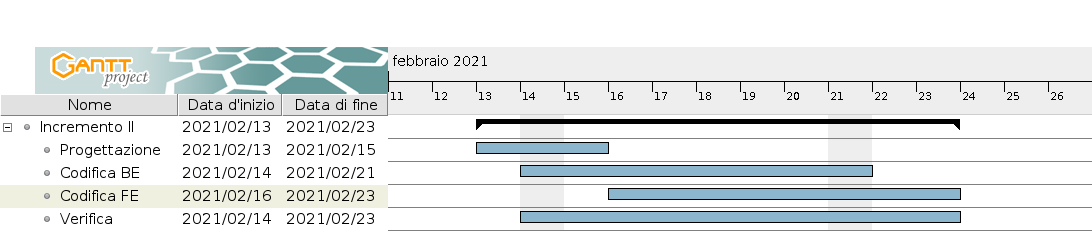
\includegraphics[width=1\linewidth]{res/images/pianificazione/incremento_2.png}
    \caption{Diagramma di Gantt dell'incremento II}
    \label{fig:_Gantt incremento II}
\end{figure}

\begin{figure}[H]
    \centering
    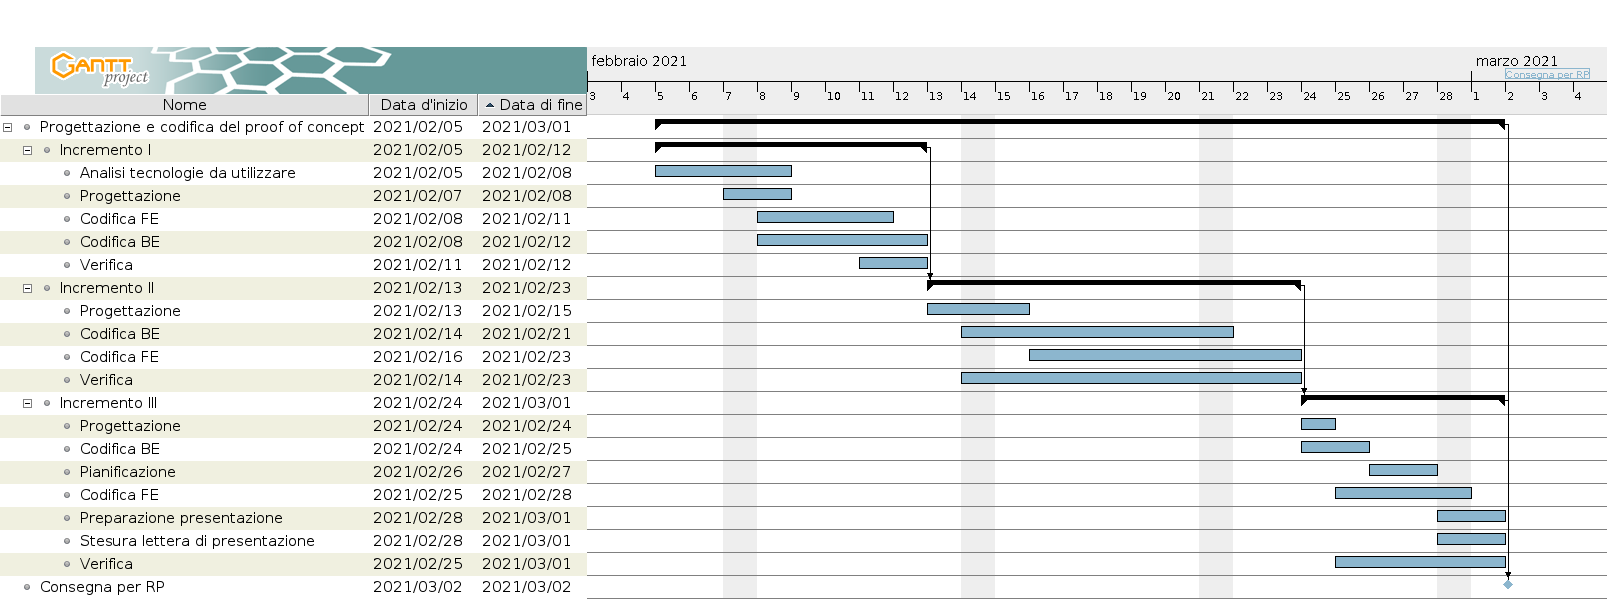
\includegraphics[width=1\linewidth]{res/images/pianificazione/progettazione_e_codifica_del_proof_of_concept.png}
    \caption{Diagramma di Gantt della fase di progettazione e codifica del proof of concept}
    \label{fig:_Gantt progettazione e codifica del proof of concept}
\end{figure}

%-------------- REVISIONE DI PROGETTAZIONE --------------

%-------------- FASE Progettazione completa e implementazione --------------

\subsection{Progettazione completa e implementazione} \label{_pianificazioneProgettazioneCompletaImplementazione}
\begin{itemize}
    \item []\textbf{Inizio:} 2021-03-02
    \item []\textbf{Fine:} 2021-04-02
    \item []\textbf{Descrizione:} effettuare una progettazione completa delle funzionalità mancanti ed effettuare una prima implementazione del prodotto.
\end{itemize}

\subsubsection{Ruoli attivi}
Durante questa fase saranno presenti i seguenti ruoli:
\begin{itemize}
    \item Responsabile;
    \item Amministratore;
    \item Analista;
    \item Progettista;
    \item Programmatore;
    \item Verificatore.
\end{itemize}

\subsubsection{Periodi e attività}

\paragraph[Incremento III]{Incremento III}
\begin{itemize}
    \item [] \textbf{Inizio:} 2021-03-02
    \item [] \textbf{Fine:} 2021-03-20
    \item [] \textbf{Attività}
          \begin{itemize}
              \item \textbf{Progettazione:} progettazione delle funzionalità non implementate nel PoC;
              \item \textbf{Analisi tecnologie da utilizzare;}
              \item \textbf{Aggiornamento della pianificazione;}
              \item \textbf{Normazione:} revisione ed eventuale aggiornamento delle norme di progetto;
              \item \textbf{Piano di qualità:} revisione ed eventuale aggiornamento del piano di qualifica;
              \item \textbf{Codifica:} codifica incrementando il PoC;
              \item \textbf{Manuale utente:} prima stesura;
              \item \textbf{Verifica:} controllo della qualità dei prodotti sviluppati in questo periodo.
          \end{itemize}
\end{itemize}

\begin{figure}[H]
    \centering
    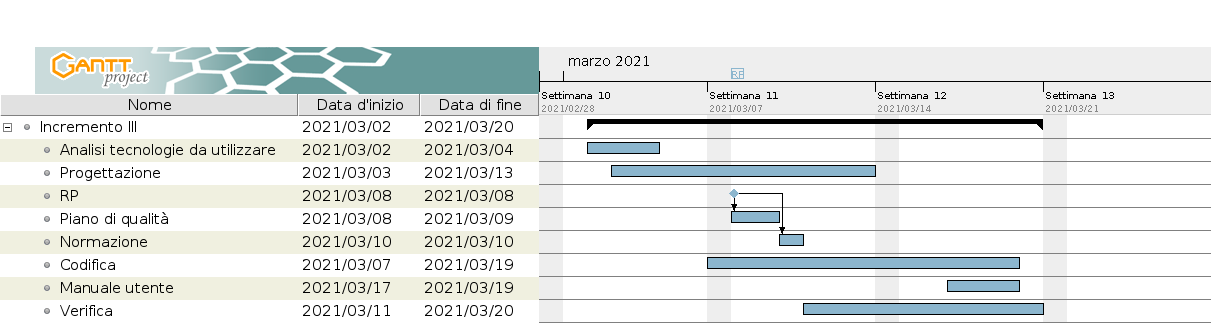
\includegraphics[width=1\linewidth]{res/images/pianificazione/incremento_3.png}
    \caption{Diagramma di Gantt dell'incremento III}
    \label{fig:_Gantt incremento III}
\end{figure}

\paragraph[Incremento IV]{Incremento IV}
\begin{itemize}
    \item [] \textbf{Inizio:} 2021-03-21
    \item [] \textbf{Fine:} 2021-04-02
    \item [] \textbf{Attività}
          \begin{itemize}
              \item \textbf{Progettazione;}
              \item \textbf{Codifica:} codifica di una prima versione del prodotto;
              \item \textbf{Manuale utente:} aggiornamento;
              \item \textbf{Preparazione presentazione:} preparazione della presentazione per la revisione di qualifica;
              \item \textbf{Stesura lettera di presentazione;}
              \item \textbf{Verifica:} controllo della qualità dei prodotti sviluppati in questo periodo.
          \end{itemize}
\end{itemize}

\begin{figure}[H]
    \centering
    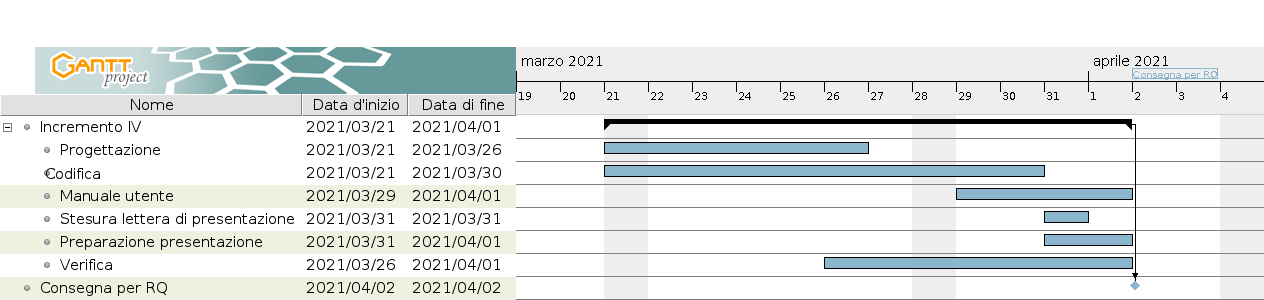
\includegraphics[width=1\linewidth]{res/images/pianificazione/incremento_4.png}
    \caption{Diagramma di Gantt dell'incremento IV}
    \label{fig:_Gantt incremento IV}
\end{figure}

\begin{figure}[H]
    \centering
    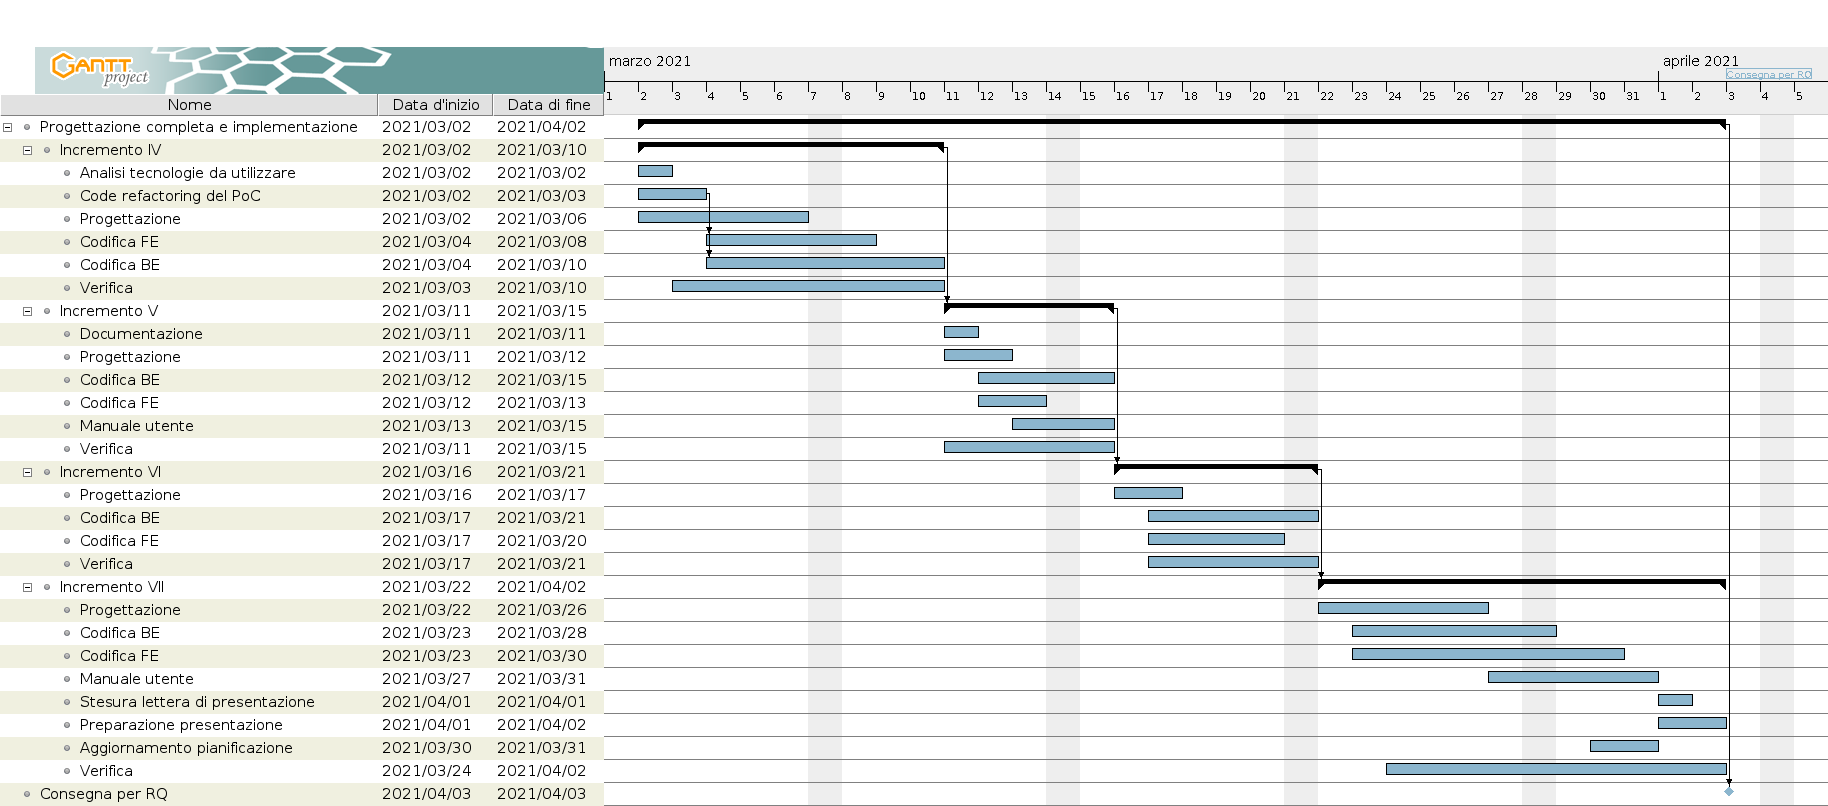
\includegraphics[width=1\linewidth]{res/images/pianificazione/progettazione_completa_e_implementazione.png}
    \caption{Diagramma di Gantt della fase di Progettazione completa e implementazione}
    \label{fig:_Gantt progettazione completa e implementazione}
\end{figure}

%-------------- REVISIONE DI QUALIFICA --------------

%-------------- FASE Termine implementazione e raffinamento generale --------------

\subsection{Termine implementazione e raffinamento generale} \label{_pianificazioneTermineImplementazione}
\begin{itemize}
    \item [] \textbf{Inizio:} 2021-04-03
    \item [] \textbf{Fine:} 2021-04-25
    \item [] \textbf{Descrizione:} completare e raffinare l'implementazione del prodotto.
\end{itemize}

\subsubsection{Ruoli attivi}
Durante questa fase saranno presenti i seguenti ruoli:
\begin{itemize}
    \item Responsabile;
    \item Amministratore;
    \item Progettista;
    \item Programmatore;
    \item Verificatore.
\end{itemize}

\subsubsection{Periodi e attività}

\paragraph[Incremento V]{Incremento V}
\begin{itemize}
    \item [] \textbf{Inizio:} 2021-04-03
    \item [] \textbf{Fine:} 2021-04-25
    \item [] \textbf{Attività}
          \begin{itemize}
              \item \textbf{Aggiornamento della pianificazione;}
              \item \textbf{Piano di qualità:} revisione ed eventuale aggiornamento del piano di qualifica;
              \item \textbf{Progettazione:} completamento;
              \item \textbf{Codifica:} fine codifica e raffinamento del prodotto;
              \item \textbf{Manuale utente:} stesura finale;
              \item \textbf{Verifica:} controllo della qualità dei prodotti sviluppati in questo periodo.
          \end{itemize}
\end{itemize}

\begin{figure}[H]
    \centering
    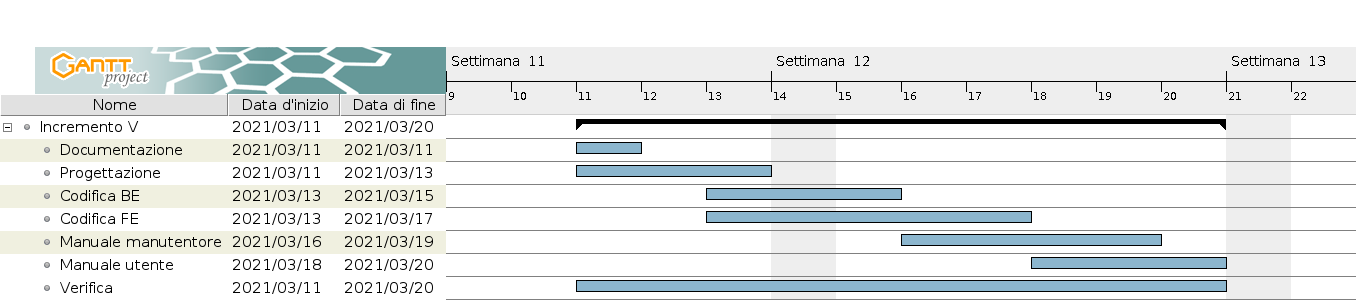
\includegraphics[width=1\linewidth]{res/images/pianificazione/incremento_5.png}
    \caption{Diagramma di Gantt dell'incremento V}
    \label{fig:_Gantt incremento V}
\end{figure}

\begin{figure}[H]
    \centering
    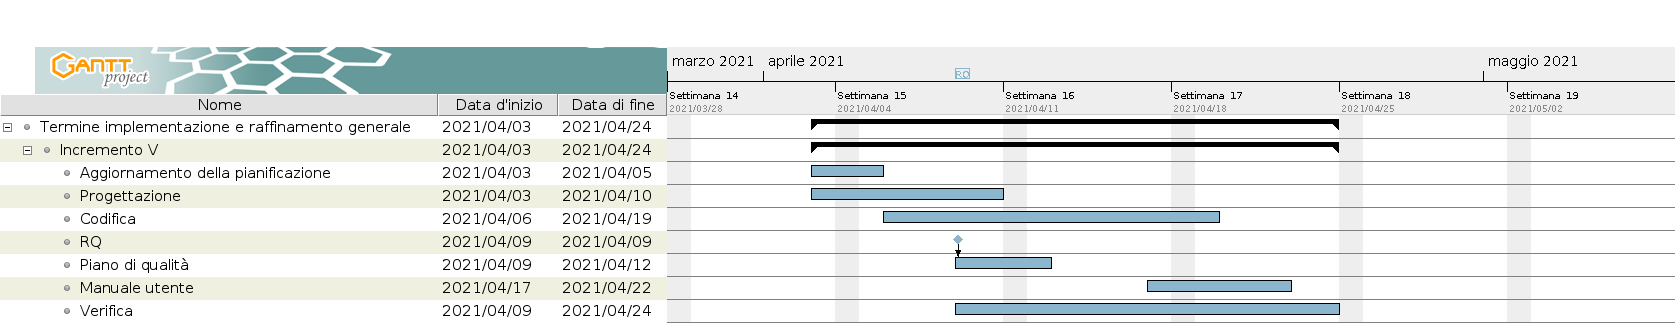
\includegraphics[width=1\linewidth]{res/images/pianificazione/termine_implementazione_e_raffinamento_generale.png}
    \caption{Diagramma di Gantt della fase di Termine implementazione e raffinamento generale}
    \label{fig:_Gantt termine implementazione e raffinamento generale}
\end{figure}

%-------------- FASE Validazione e collaudo --------------

\subsection{Validazione e collaudo} \label{_pianificazioneValidazioneCollaudo}
\begin{itemize}
    \item [] \textbf{Inizio:} 2021-04-26
    \item [] \textbf{Fine:} 2021-05-10
    \item [] \textbf{Descrizione:} verificare e collaudare il prodotto.
\end{itemize}

\subsubsection{Ruoli attivi}
Durante questa fase saranno presenti i seguenti ruoli:
\begin{itemize}
    \item Responsabile;
    \item Amministratore;
    \item Progettista;
    \item Programmatore;
    \item Verificatore.
\end{itemize}

\subsubsection{Periodi e attività}

\paragraph[Unico periodo]{Unico periodo}
\begin{itemize}
    \item [] \textbf{Inizio:} 2021-04-20
    \item [] \textbf{Fine:} 2021-05-10
    \item [] \textbf{Attività}
          \begin{itemize}
              \item \textbf{Aggiornamento della pianificazione;}
              \item \textbf{Codifica:} rilascio ultima versione;
              \item \textbf{Manuale utente:} revisione ed eventuale aggiornamento;
              \item \textbf{Preparazione presentazione:} preparazione della presentazione per la revisione di accettazione;
              \item \textbf{Stesura lettera di presentazione;}
              \item \textbf{Verifica:} controllo della qualità dei prodotti sviluppati in questo periodo.
          \end{itemize}
\end{itemize}

\begin{figure}[H]
    \centering
    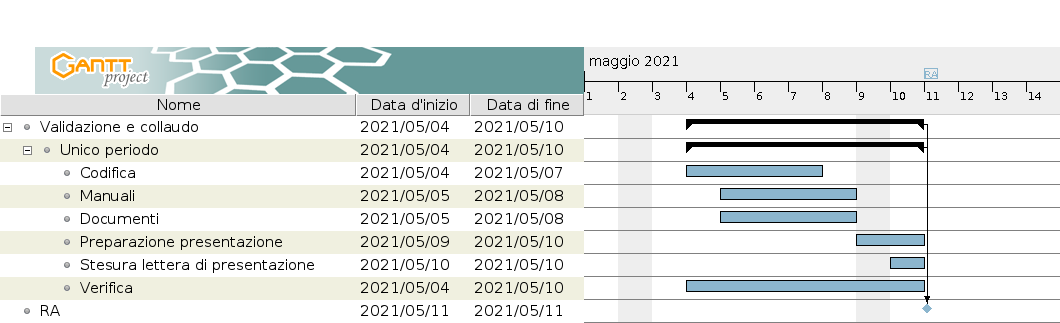
\includegraphics[width=1\linewidth]{res/images/pianificazione/validazione_e_collaudo.png}
    \caption{Diagramma di Gantt della fase di Validazione e collaudo}
    \label{fig:_Gantt Validazione e collaudo}
\end{figure}

%-------------- REVISIONE DI ACCETTAZIONE --------------